\section{Parallel Performance}
\label{sec:parallel performance}

This section presents two laws that aim to describe two different things when discussing performance speed up.
The first is Amdahl's Law which describes how much faster a program can become with the same workload, and the second is Gustafson-Barsis Law which describes how much more work can be performed with the same running time.
However, neither take into account that all computations have some overhead, e.g. reading and writing data, atomic operations where threads wait for each other, creating or deleting threads, etc.

\subsection{Amdahl's Law}
\label{sec:amdahls law}

Amdahl's Law is an equation that aims to approximate the potential speed up of a serial program.
The equation is presented in \cref{eq:amdahls law}, where $P$ is the portion of the serial code that can be parallelized, $(1-P)$ is the portion that cannot be made parallel, and we have $n$ processors.
Thus, $S(n)$ approximates the speed up by making a program parallel.

\begin{equation}
  \label{eq:amdahls law}
  S(n) = \frac{1}{(1-P) + P/n}
\end{equation}

Amdahl's Law only applies if the amount of work performed in the parallel version is not significantly different than the serial code's amount of work.
An illustration of the potential speed up is presented in \cref{fig:amdahls law} with $n=1024$.
It shows that the optimal solution is that the entire portion of code can be made parallel, and the code runs $n$ times faster compared to the serial code, when running $n$ processors~\cite{farber2011cuda}.

\begin{figure}[htb]
  \centering
  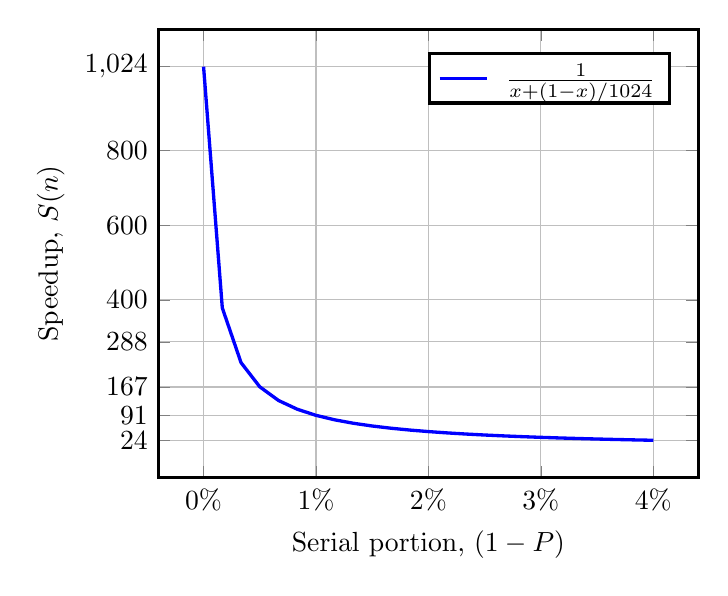
\begin{tikzpicture}
  \begin{axis}[
    ymajorgrids,
    xmajorgrids,
    ylabel={Speedup, $S(n)$},
    ytick={24,91,167,288,400,600,800,1024},
    xlabel={Serial portion, $(1-P)$},
    scaled x ticks = false, % do not add axis-multiplier
    xticklabel={% print percent
      \pgfmathparse{\tick*100}%
      \pgfmathprintnumber{\pgfmathresult}%
      \%%
    },
    legend style={
      at={(0.95,0.95)},
      anchor=north east,
      column sep=1ex
     },
     no markers,
     very thick
  ]

  \addplot+[domain=0.00:0.04] {1/(x+((1-x)/1024))};
  \addlegendentry{$\frac{1}{x + (1-x) / 1024}$};
  \end{axis}
\end{tikzpicture}

  \caption{Speed up given by Amdahl's Law with variable portions of code that can be made parallel $P$ and $n=1024$ processors}
  \label{fig:amdahls law}
\end{figure}

Notice how steep the curve is when the serial portion moves from 1\% to 0\%.
With 1\% serial portion the speed up is about $91\times$, and $1024\times$ when everything can be made parallel.
According to Amdahl's Law, with just a tiny portion of the code that cannot become parallel, a high speed up is not likely to be achieved.

\subsection{Gustafson-Barsis Law}
\label{sec:gustafson-barsis law}

The point that Gustafson makes is that many computational problems scale with the number of processors available, e.g. computing pi -- if we have more computational power, we compute more digits of pi~\cite{amdahlorgustafson2011}.
Note, however that if the goal at hand is to compute pi quicker, then that is of course possible, this is just not what Gustafson-Barsis Law aims to describe.

\begin{equation}
  \label{eq:gustafson-barsis law}
  W(n) = n + (1-n) \times (1-P)
\end{equation}

So, the goal is to run a program in the same amount of time but with more work.
This approximation is present in \cref{eq:gustafson-barsis law}.
Thus, $W(n)$ gives the amount of work that can be further performed~\cite{gustafson1988reevaluating}.

